%% (Master) Thesis template
% Template version used: v1.4
%
% Largely adapted from Adrian Nievergelt's template for the ADPS
% (lecture notes) project.


%% We use the memoir class because it offers a many easy to use features.
\documentclass[11pt,a4paper,titlepage]{memoir}

%% Packages
%% ========

%% LaTeX Font encoding -- DO NOT CHANGE
\usepackage[OT1]{fontenc}

%% Babel provides support for languages.  'english' uses British
%% English hyphenation and text snippets like "Figure" and
%% "Theorem". Use the option 'ngerman' if your document is in German.
%% Use 'american' for American English.  Note that if you change this,
%% the next LaTeX run may show spurious errors.  Simply run it again.
%% If they persist, remove the .aux file and try again.
\usepackage[english]{babel}

%% Input encoding 'utf8'. In some cases you might need 'utf8x' for
%% extra symbols. Not all editors, especially on Windows, are UTF-8
%% capable, so you may want to use 'latin1' instead.
\usepackage[utf8]{inputenc}

%% This changes default fonts for both text and math mode to use Herman Zapfs
%% excellent Palatino font.  Do not change this.
\usepackage[sc]{mathpazo}

%% The AMS-LaTeX extensions for mathematical typesetting.  Do not
%% remove.
\usepackage{amsmath,amssymb,amsfonts,mathrsfs}

%% NTheorem is a reimplementation of the AMS Theorem package. This
%% will allow us to typeset theorems like examples, proofs and
%% similar.  Do not remove.
%% NOTE: Must be loaded AFTER amsmath, or the \qed placement will
%% break
\usepackage[amsmath,thmmarks]{ntheorem}

%% LaTeX' own graphics handling
\usepackage{graphicx}

%% We unfortunately need this for the Rules chapter.  Remove it
%% afterwards; or at least NEVER use its underlining features.
\usepackage{soul}

%% This allows you to add .pdf files. It is used to add the
%% declaration of originality.
\usepackage{pdfpages}

%% Some more packages that you may want to use.  Have a look at the
%% file, and consult the package docs for each.
%% See the TeXed file for more explanations

%% [OPT] Multi-rowed cells in tabulars
%\usepackage{multirow}

%% [REC] Intelligent cross reference package. This allows for nice
%% combined references that include the reference and a hint to where
%% to look for it.
\usepackage{varioref}

%% [OPT] Easily changeable quotes with \enquote{Text}
%\usepackage[german=swiss]{csquotes}

%% [REC] Format dates and time depending on locale
\usepackage{datetime}

%% [OPT] Provides a \cancel{} command to stroke through mathematics.
%\usepackage{cancel}

%% [NEED] This allows for additional typesetting tools in mathmode.
%% See its excellent documentation.
\usepackage{mathtools}

%% [ADV] Conditional commands
%\usepackage{ifthen}

%% [OPT] Manual large braces or other delimiters.
%\usepackage{bigdelim, bigstrut}

%% [REC] Alternate vector arrows. Use the command \vv{} to get scaled
%% vector arrows.
\usepackage[h]{esvect}

%% [NEED] Some extensions to tabulars and array environments.
\usepackage{array}

%% [OPT] Postscript support via pstricks graphics package. Very
%% diverse applications.
%\usepackage{pstricks,pst-all}

%% [?] This seems to allow us to define some additional counters.
%\usepackage{etex}

%% [ADV] XY-Pic to typeset some matrix-style graphics
%\usepackage[all]{xy}

%% [OPT] This is needed to generate an index at the end of the
%% document.
%\usepackage{makeidx}

%% [OPT] Fancy package for source code listings.  The template text
%% needs it for some LaTeX snippets; remove/adapt the \lstset when you
%% remove the template content.
\usepackage{listings}
\lstset{language=TeX,basicstyle={\normalfont\ttfamily}}

%% [REC] Fancy character protrusion.  Must be loaded after all fonts.
\usepackage[activate]{pdfcprot}

%% [REC] Nicer tables.  Read the excellent documentation.
\usepackage{booktabs}


%% Our layout configuration.  DO NOT CHANGE.
%% Memoir layout setup

%% NOTE: You are strongly advised not to change any of them unless you
%% know what you are doing.  These settings strongly interact in the
%% final look of the document.

% Dependencies
\usepackage{ETHlogo}

% Turn extra space before chapter headings off.
\setlength{\beforechapskip}{0pt}

\nonzeroparskip
\parindent=0pt
\defaultlists

% Chapter style redefinition
\makeatletter

\if@twoside
  \pagestyle{Ruled}
  \copypagestyle{chapter}{Ruled}
\else
  \pagestyle{ruled}
  \copypagestyle{chapter}{ruled}
\fi
\makeoddhead{chapter}{}{}{}
\makeevenhead{chapter}{}{}{}
\makeheadrule{chapter}{\textwidth}{0pt}
\copypagestyle{abstract}{empty}

\makechapterstyle{bianchimod}{%
  \chapterstyle{default}
  \renewcommand*{\chapnamefont}{\normalfont\Large\sffamily}
  \renewcommand*{\chapnumfont}{\normalfont\Large\sffamily}
  \renewcommand*{\printchaptername}{%
    \chapnamefont\centering\@chapapp}
  \renewcommand*{\printchapternum}{\chapnumfont {\thechapter}}
  \renewcommand*{\chaptitlefont}{\normalfont\huge\sffamily}
  \renewcommand*{\printchaptertitle}[1]{%
    \hrule\vskip\onelineskip \centering \chaptitlefont\textbf{\vphantom{gyM}##1}\par}
  \renewcommand*{\afterchaptertitle}{\vskip\onelineskip \hrule\vskip
    \afterchapskip}
  \renewcommand*{\printchapternonum}{%
    \vphantom{\chapnumfont {9}}\afterchapternum}}

% Use the newly defined style
\chapterstyle{bianchimod}

\setsecheadstyle{\Large\bfseries\sffamily}
\setsubsecheadstyle{\large\bfseries\sffamily}
\setsubsubsecheadstyle{\bfseries\sffamily}
\setparaheadstyle{\normalsize\bfseries\sffamily}
\setsubparaheadstyle{\normalsize\itshape\sffamily}
\setsubparaindent{0pt}

% Set captions to a more separated style for clearness
\captionnamefont{\sffamily\bfseries\footnotesize}
\captiontitlefont{\sffamily\footnotesize}
\setlength{\intextsep}{16pt}
\setlength{\belowcaptionskip}{1pt}

% Set section and TOC numbering depth to subsection
\setsecnumdepth{subsection}
\settocdepth{subsection}

%% Titlepage adjustments
\pretitle{\vspace{0pt plus 0.7fill}\begin{center}\HUGE\sffamily\bfseries}
\posttitle{\end{center}\par}
\preauthor{\par\begin{center}\let\and\\\Large\sffamily}
\postauthor{\end{center}}
\predate{\par\begin{center}\Large\sffamily}
\postdate{\end{center}}

\def\@advisors{}
\newcommand{\advisors}[1]{\def\@advisors{#1}}
\def\@department{}
\newcommand{\department}[1]{\def\@department{#1}}
\def\@thesistype{}
\newcommand{\thesistype}[1]{\def\@thesistype{#1}}

\renewcommand{\maketitlehooka}{\noindent\ETHlogo[2in]}

\renewcommand{\maketitlehookb}{\vspace{1in}%
  \par\begin{center}\Large\sffamily\@thesistype\end{center}}

\renewcommand{\maketitlehookd}{%
  \vfill\par
  \begin{flushright}
    \sffamily
    \@advisors\par
    \@department, ETH Z\"urich
  \end{flushright}
}

\checkandfixthelayout

\setlength{\droptitle}{-48pt}

\makeatother

% This defines how theorems should look. Best leave as is.
\theoremstyle{plain}
\setlength\theorempostskipamount{0pt}

%%% Local Variables:
%%% mode: latex
%%% TeX-master: "thesis"
%%% End:


%% Theorem environments.  You will have to adapt this for a German
%% thesis.
%% Theorem-like environments

%% This can be changed according to language. You can comment out the ones you
%% don't need.

\numberwithin{equation}{chapter}

%% German theorems
%\newtheorem{satz}{Satz}[chapter]
%\newtheorem{beispiel}[satz]{Beispiel}
%\newtheorem{bemerkung}[satz]{Bemerkung}
%\newtheorem{korrolar}[satz]{Korrolar}
%\newtheorem{definition}[satz]{Definition}
%\newtheorem{lemma}[satz]{Lemma}
%\newtheorem{proposition}[satz]{Proposition}

%% English variants
\newtheorem{theorem}{Theorem}[chapter]
\newtheorem{example}[theorem]{Example}
\newtheorem{remark}[theorem]{Remark}
\newtheorem{corollary}[theorem]{Corollary}
\newtheorem{definition}[theorem]{Definition}
\newtheorem{lemma}[theorem]{Lemma}
\newtheorem{proposition}[theorem]{Proposition}

%% Proof environment with a small square as a "qed" symbol
\theoremstyle{nonumberplain}
\theorembodyfont{\normalfont}
\theoremsymbol{\ensuremath{\square}}
\newtheorem{proof}{Proof}
%\newtheorem{beweis}{Beweis}


%% Helpful macros.
%% Custom commands
%% ===============

%% Special characters for number sets, e.g. real or complex numbers.
\newcommand{\C}{\mathbb{C}}
\newcommand{\K}{\mathbb{K}}
\newcommand{\N}{\mathbb{N}}
\newcommand{\Q}{\mathbb{Q}}
\newcommand{\R}{\mathbb{R}}
\newcommand{\Z}{\mathbb{Z}}
\newcommand{\X}{\mathbb{X}}

%% Fixed/scaling delimiter examples (see mathtools documentation)
\DeclarePairedDelimiter\abs{\lvert}{\rvert}
\DeclarePairedDelimiter\norm{\lVert}{\rVert}

%% Use the alternative epsilon per default and define the old one as \oldepsilon
\let\oldepsilon\epsilon
\renewcommand{\epsilon}{\ensuremath\varepsilon}

%% Also set the alternate phi as default.
\let\oldphi\phi
\renewcommand{\phi}{\ensuremath{\varphi}}


%% Make document internal hyperlinks wherever possible. (TOC, references)
%% This MUST be loaded after varioref, which is loaded in 'extrapackages'
%% above.  We just load it last to be safe.
\usepackage[linkcolor=black,colorlinks=true,citecolor=black,filecolor=black]{hyperref}

%% This is an additional package for scientific bibliographic representation
\usepackage[numbers]{natbib}

%% Document information
%% ====================

%\title{A Secure, Isolated and Air-Gapped Signing System}
\title{SIAGSS and the Formal Verification of Signing Ceremonies}
\author{Fabian Andreas Murer}
\thesistype{Master Thesis}
\advisors{Advisors: Prof.\ Dr.\ Adrian Perrig, Brian Trammell}
\department{Department of Computer Science}
\date{April 4, 2018}

\begin{document}

\frontmatter

%% Title page is autogenerated from document information above.  DO
%% NOT CHANGE.
\begin{titlingpage}
  \calccentering{\unitlength}
  \begin{adjustwidth*}{\unitlength-24pt}{-\unitlength-24pt}
    \maketitle
  \end{adjustwidth*}
\end{titlingpage}

%% The abstract of your thesis.  Edit the file as needed.
\begin{abstract}
Keeping the signing key save and secure is a crucial part in the public key infrastructure (PKI). If an attacker manages to steal a signing key, he is able to sign requests by himself and making everyone believe that this request has been certified by the original key holder. The goal of this thesis is to develop a new approach how to store a signing key in an isolated environment, still being able to accept and sign requests. We achieve this by using an air-gapped channel and two subsystems, where one of them is completely isolated from any network, has reduced to no radio frequency emissions and in the optimal case not even attached directly to a power supply. The whole system should be able to handle a fair amount of requests a day while still be of relative low cost. Furthermore, we want to formally verify ceremonies when initialising, changing or backing up secret keys.
\end{abstract}


%% TOC with the proper setup, do not change.
\cleartorecto
\tableofcontents
\mainmatter

\lstnewenvironment{code}[1][]%
  {\noindent\minipage{\textwidth}\medskip 
   \lstset{basicstyle=\ttfamily\footnotesize,
   frame=single,
   showstringspaces=false,
   commentstyle=\color{red},
   keywordstyle=\color{blue},
   captionpos=b,
   #1}}
  {\endminipage}
  
%% Your real content!
% Some commands used in this file
\newcommand{\package}{\emph}

\chapter{Introduction}\label{chapter:intro}
For hundreds of years, people have been using signatures, typically to bind a person to a contract. Since the digital age, digital signatures have appeared which basically have the same ulterior motivates, i.e., binding two objects to each other. Typical examples are binding a name to a person or a name to an IP-address like it is done in the \emph{Domain Name Security Extensions} (DNSSEC). Such signing mechanisms most likely use a \emph{public key infrastructure} (PKI). The very crucial part in every system that uses PKI is to keep the private/signing key secure. This not always an easy task to solve, as a system where the signing key is stored might be compromised or even stolen physically. One goal of this thesis is to figure out if it is possible to build a rather simple signing system that is located in a totally isolated and safe environment such that it can be used to sign assertions (e.g., the mapping of a name to an address) over an air-gapped channel. Based on the idea of \citet{castle}, the air-gapped channel will consist of two monitors standing in front of each other and two cameras pointing to the opposite monitor. The reason why we want to use such a visual air-gap is that one can easily monitor and audit what happens on the screens, i.e., on the channel. Furthermore, the system should be of relatively low cost and yet effective, since this system will mainly be used to sign assertions from the RAINS protocol used in the new Internet architecture SCION \cite{scion_book}, where a lot of requests have to be handled.

Sometimes, managing secret keys like the signing key needs involvement of a human being. While a protocol implemented in a program simply follows the steps that it needs to do, a human can make mistakes, e.g., leave some step out or lose some key. The \emph{control-plane PKI} of SCION \cite{scion_book} uses an \emph{online} and \emph{offline} asymmetric key pair. While the online key is used for frequent mechanisms, the offline keys are used for infrequent and safety critical operations like adding or removing a core AS to the \emph{Trust Root Configuration} (TRC). Unlike the automated use of online keys, the use of offline keys needs interaction with an administrator. Since no human is perfect, even a trained administrator can make mistakes. For this reason, the second goal of this thesis is to formally verify key ceremonies based on the work of \citet{basin2016modeling}. By modeling the ceremonies including human interaction, we want to verify a safe and secure execution of the protocol despite the existence of fallible humans.

In the first part of this thesis we want to describe the signing system, how it is composed, how it works and what is needed to operate it. This is followed by discussing the key management of the signing system in \autoref{chapter:key_management}. In \autoref{chapter:formal_verification} we start describing the protocol of a ceremony, followed by modeling and verifying it.
\chapter{Signing System}\label{chapter:system}
In this chapter we want to describe the actual signing system, it's parts and how it works. Furthermore, this chapter includes advices how to use the system correctly and how to deploy it secure and in isolation.

\section{Idea}\label{sec:idea}
Before we start describing the system, we first want to elaborate the idea behind the system. The idea is based on the system from \citet{castle}. In their project, they had one system component that stands in an isolated glass box. The system is equipped with a monitor and a camera. Now the only channel to and from this box is an air-gapped channel based on this monitor and camera. All the data that needs to be exchanged is encoded into a QR-code and read by cameras from the screen. In \cite{castle}, the interaction with the isolated box only happens with human interaction, i.e., system administrators come and scan the QR-code from the monitor and show their own QR-codes to the system.

Unlike \cite{castle}, we use two components that do not need any human interaction except of the initialization process. The main thought here is that we use the idea of \cite{castle} to create a signing machine which is completely isolated. The second part of the system is used to receive requests from different outsiders and convert the requests to QR-codes readable by the signing component.

\begin{figure}
\centering
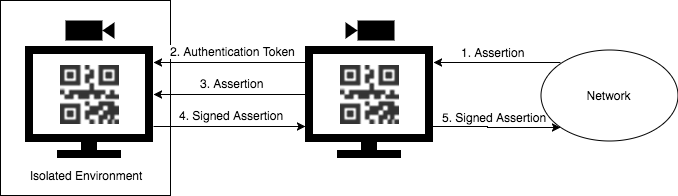
\includegraphics[width=0.8\textwidth]{images/SystemOverview.png}
\caption{This image shows a basic overview of the system components and how they interact.}
\label{fig:overview}
\end{figure}

\section{Requirements}\label{sec:requirements}
This section states the different requirements on the signing system, starting with the functional requirements followed by the non-functional requirements.

\subsection{Functional Requirements}\label{subsec:functional}
Let us start with the functional requirements of the system. The general goal of the system is to receive requests from the network containing some data. This data needs to be transfered over an air-gapped channel, signed and transfered back over the air-gapped channel and back to the network. As we have already described the idea before, this is done by using QR-codes and displaying and reading them from a screen respectively. So the system needs to be able to

\begin{enumerate}
\item receive requests from the network,
\item queue the incoming requests and handle them in \emph{first come first serve} manner,
\item encode requests in a QR-code and display the QR-code on a screen,
\item read the QR-code from a screen using a camera,
\item decode the QR-code and get its data,
\item sign the data using the \emph{Curve25519 Algorithm} \citep{bernstein2012high},
\item send the signed request back to the originating sender
\end{enumerate}

Furthermore, in order to avoid an adversary injecting some other data and getting it signed, the system needs to be able to authenticate the requests and thus only sign authenticated requests. Moreover, the system needs to be able to generate new public/private key pairs and to distribute the public keys.


\subsection{Non-Functional Requirements}\label{subse:non-functional}
After describing the functional requirements, let us concentrate on the non-functional requirements. As we have already mentioned in \autoref{sec:idea}, one part of the system needs to be isolated as much as possible. In more detail, this means

\begin{enumerate}
\item \emph{no} Internet connection,
\item \emph{no} emitting radiation (Bluetooth, WiFi, etc.),
\item \emph{no} direct connection to a power supply (in the ideal case)
\end{enumerate}

where the last point could be achieved by charging the device over induction. Furthermore, the secret/signing keys need to be kept secret and should \emph{never} leave the signing machine.

Since there is no certificate revocation in the SCION architecture \cite{scion_book} and they are using short lived certificates instead, there will be a lot of signing requests. An optimistic counting would yield in $2$ million signatures a day, which is around $23$ signatures a second. So in the ideal case, the system should be able to handle at least that amount of requests.

Moreover, in order to display and read the QR-codes, the System needs to have two screens as well as two cameras. Also, since the system is web-based as we will see in \autoref{sec:components}, the system must run on a recent browser like Google Chrome.


\section{System Components}\label{sec:components}
We have now seen the system's requirements, so let us now describe the system itself. As already mentioned in \autoref{sec:idea}, the system mainly consists of two components. This is also visible in \autoref{fig:overview}, which shows a very basic overview of the system and how the components interact with each other. There, one can see the two main components. First on the left side in the isolated environment we have the signing system, we call it the \emph{Signer}. The Signer is responsible for receiving and signing requests from the second component in the middle of \autoref{fig:overview}, which we call the \emph{Signee}. The Signee receives requests from the network and transforms the requests into readable objects for the signer. Notice here, that points 2 and 3, i.e., authentication and sending the assertion, happens in the same message (see in \autoref{fig:signee}).

In the following sections we want to describe the two components in more detail. Both components are running \texttt{Node.js}\footnote{Node.js: \url{https://nodejs.org/en/}} in version $8.6.0$. In order to read and decode the QR-codes, generate QR-codes and sign the requests, we used the following external libraries:

\begin{description}
\item[Instascan:] We used the Node module called \texttt{Instascan} from \citet{instascan} to read and decode the QR-code from a monitor. This module makes it easy to select a provided camera, e.g. the internal webcam of a laptop, and add a listener that returns the content of the QR-code once the scanner has read and decoded one.
\item[jQuery-qrcode:] Unfortunately, the Instascan module does not provide a method to generate a QR-code, so we used a plug-in for \texttt{jQuery} provided by \citet{jqueryqrcode}. This allows to use simple \texttt{jQuery}-method calls to generate a new QR-code.
\item[TweetNaCl:] In order to match the signing algorithm used in SCION \cite{scion_book}, namely the algorithm called \emph{ed25519} based on elliptic curves and introduced by \citet{bernstein2012high}, we used the Node module called \texttt{TweetNaCl} from \citet{tweetnacl}.
\end{description}


\subsection{The Signee System}\label{subsec:signee}

\begin{figure}
\centering
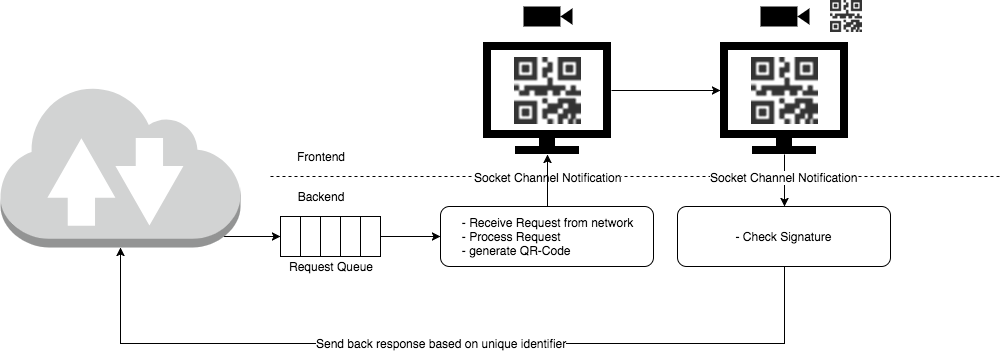
\includegraphics[width=0.8\textwidth]{images/Signee.png}
\caption{This figure shows a general overview of the \emph{Signee}}
\label{fig:signee}
\end{figure}

In this section we want to describe the first part of the system that a request reaches, namely the \emph{Signee}. The Signee listens on a predefined port (default port is $3000$) for \texttt{POST} requests containing data that needs to be signed by the \emph{Signer}. Thereby, the request needs to have the following parameters:

\begin{code}[caption={Expected message format when sending a new request to the Signee}]
data=DATA_TO_SIGN&from=VALID_FROM&to=VALID_TO
\end{code}

where DATA\_TO\_SIGN stands for the actual data that needs to be signed by the Signer, for example an assertion for a name resolution. The parameters $from$ and $to$ describe the desired validity range. Notice, that it is the desired validity range and that the Signer checks whether it is a valid range or not (more on this later).

Once a request is received, the Signee puts it in a queue, together with a callback to a request handler. Every request in the queue is then handled in \emph{first in first out} (FIFO) order. In order to hinder an adversary to inject any irregular request, every request gets authenticated by appending the \texttt{HMAC} of the data to the request. We use the \texttt{HMAC} module from the Node.js crypto library\footnote{Node.js Crypto Library: \url{https://nodejs.org/api/crypto.html}} to achieve this. The request is then sent to the front-end, i.e., the browser, using \emph{Socket Notifications}. Notice that the system expects a specific \texttt{JSON} format like in \autoref{listing:signee_to_signer}. Moreover, notice the unique identification number. This identification number is computed by calculating the hash of the request. The ID is used to reference back to the original request such that the Signee is able to return to the right requester later on.

\begin{code}[caption={Expected message format from the Signee to the Signer}, label={listing:signee_to_signer}]
{
    id: UNIQUE_ID,
    data: { data: DATA_TO_SIGN,
            from: VALID_FROM,
            to: VALID_TO },
    mac: HMAC_OF_DATA
}
\end{code}

The browser then encodes this information into a QR-code using the \emph{jQuery plug-in} mentioned before.

Once the Signee scans a new QR-code from the Signer's screen, the browser decodes it and sends the decoded content back to the back-end again using \emph{Socket Notifications}. The Signee then checks whether the signature is indeed from the expected Signer and if yes, it sends the signed data back to its origin. In order to handle the right request and response objects, the Signee uses the unique id which it has computed before. The final response has the format like in \autoref{listing:signee_to_origin}.

\begin{code}[caption={Expected message format from the Signee back to the origin}, label={listing:signee_to_origin}]
{
    assertion: { data: DATA_TO_SIGN,
                 valid_from: DATE_IN_UTC_FORMAT,
                 valid_until: DATE_IN_UTC_FORMAT },
    signature: SIGNATURE_OF_ASSERTION
}
\end{code}

You can find a graphical overview of the Signee in \autoref{fig:signee}. This overview shows the very high-level interaction between the front-end and the back-end of the Signee.


\subsection{The Signer System}

\begin{figure}
\centering
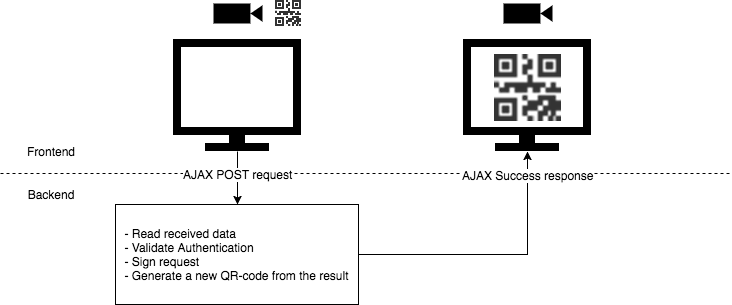
\includegraphics[width=0.8\textwidth]{images/Signer.png}
\caption{This figure shows a general overview of the \emph{Signer}}
\label{fig:signer}
\end{figure}

After having covered the Signee, we now want to describe the second component of the system, namely the \emph{Signer}. Similar to the Signee, the Signer runs a Node.js server. However, unlike the Signee, the Signer gets its requests not from the network, but reads it from the Signee's screen. One reason for this is the requirement that the Signer needs to be totally isolated and therefore can not be connected to any network. In order to read the QR-code from the Signee's screen, the Signer also uses the Instascan module as described before. Once the QR-code has been read and decoded by the module, the content is sent to the back-end using an \texttt{AJAX POST request}. The back-end first verifies the authentication token, i.e., checking the hash of the data against the received hash-value. If it is correct, the Signer extracts the data from the request and checks the validity range. Thereby, the starting date must start in the future and the duration must not be longer than a predefined maximum value. If the validity range is valid, the Signer signs the data together with the validity range.

\begin{code}[caption={Expected message format from the Signer back to the Signee}, label={listing:signer_to_signee}]
{
    id: UNIQUE_ID,
    assertion: { data: DATA_TO_SIGN,
                 valid_from: DATE_IN_UTC_FORMAT,
                 valid_until: DATE_IN_UTC_FORMAT },
    signature: SIGNATURE_OF_ASSERTION },
}
\end{code}

The result is then sent back to the front-end using success callback of the \texttt{AJAX} request using the format in \autoref{listing:signer_to_signee}. In the front-end, the response is encoded into a QR-code and displayed on the screen for the Signee to read it. The important part here is that the Signer sends back the request identifier so that the Signee can redirect the signed data to the right originator. 

\autoref{fig:signer} shows a graphical overview of the interaction between the front-end and the back-end of the Signer.

\section{System Setup}\label{sec:setup}
Now that we have described the two system components, we want show our prototype setup. For our prototype setup we first met the assumption of complete isolation of the Signer system, i.e., we did not especially shield or isolate the system. However, we argue that since the system implementation does not need any Internet connection or some other connection, we could simply use the method of \cite{castle} in order to make the Signer running in an isolated environment.

% TODO: name specific laptop specification
The overall system setup is very minimalistic. For each of the two components we simply used a commodity laptop. For the Signer we used a HP Aspire and for the Signee a Lenovo Thinkpad. Both laptops run a clean install of Ubuntu $16.04.3$ LTS with the Google Chrome Browser and Node.js Server installed additionally.

\subsection{Initialization}
Before the system is ready to run correctly, both components need first to be initialized. The initialization includes downloading the corresponding source code and then in a next step installing the needed \emph{node-modules}. The best way to do this is to simply run \texttt{npm install}. Notice that one will need the \texttt{package.json} file (see \autoref{listing:package_json}) from the repository\footnote{GitHub Repository: \url{https://github.com/fmurer/master_thesis}}.

\begin{code}[caption={Example \texttt{package.json} containing the needed node-modules}, label={listing:package_json}]
{
  "name": "signer",
  "version": "1.0.0",
  "description": "",
  "main": "app.js",
  "scripts": {
    "test": "echo \"Error: no test specified\" && exit 1"
  },
  "author": "Fabian Murer",
  "license": "ISC",
  "dependencies": {
    "express": "^4.16.2",
    "jquery": "^3.2.1",
    "morgan": "^1.9.0",
    "node-schedule": "^1.2.5",
    "qrcode-generator": "^1.3.1",
    "socket.io": "^2.0.4",
    "tweetnacl": "^1.0.0"
  }
}
\end{code}

Next to installing the modules from \texttt{package.json}, one also needs to install \emph{Instascan} \cite{instascan} and the \emph{jQuery plug-in} \cite{jqueryqrcode} for generating the QR-codes. Furthermore, a system administrator needs to place the Signer's public key on the Signee before starting the system, otherwise the Signee fails to verify the responses from the Signer. For the initial key generation, a script is provided (see \autoref{listing:key_gen}). So the administrator only needs to put the file \texttt{signer.pub} onto the Signee.

\begin{code}[language=bash, breaklines=true, caption={Script for initial key pair generation}, label={listing:key_gen}]
#!/bin/bash

keypair="$(node -e 'keyPair = require("../signer/node_modules/tweetnacl").sign.keyPair();
console.log(Buffer.from(keyPair.publicKey).toString("hex"));
console.log(Buffer.from(keyPair.secretKey).toString("hex"));
console.log("");')"

echo "${keypair}"

counter=0
while IFS='' read -r line || [[ -n "$line" ]]; do
	echo "$line" > key_"$counter"
	let counter++
done <<< "${keypair}"

mv ./key_0 ../signer/pk/signer.pub
mv ./key_1 ../signer/sk/sign_key
\end{code}

After having installed all the needed modules, the system administrator should also manually launch the pairing of the systems by pressing the $p$ button on the Signee's keyboard. This guarantees an initial shared secret between the Signer and the Signee which is then used for authenticating the messages sent from the Signee to the Signer.


\subsection{Running Example}
Once everything is initialized according to what we have seen before, the rest of the setup is really simple. The two laptops need to be placed opposed to each other such that the camera of the Signee can see the monitor of the Signer and vice versa.

\begin{description}
\item[Remark:] \textit{One thing that came across while implementing and testing the system was that a too bright monitor makes the camera unable to read the QR-code from it, because the white parts outshine the dark parts. So in order for the cameras to read properly, the brightness needs to be adjusted accordingly. In the current setup with the two laptops, this means reducing the screen brightness to maximum $50\%$.}
\end{description}

This is already all for a basic example. The only thing left is to start both servers with \texttt{node app.js}. Now one can send \texttt{POST} requests using the format mentioned in \autoref{subsec:signee} and send it to the Signee on the specific port (default is port $3000$). \autoref{fig:prototype} shows a running example including a view on the monitors.

\begin{figure}
\centering
%\includegraphics[width=0.8\textwidth]{}
\caption{Example setup of the prototype showing the monitors while running}
\label{fig:prototype}
\end{figure}








\chapter{Environment}\label{chapter:environment}
In this chapter we want to describe the environment in which the system will be placed. This includes assumptions about the location like the building and the server room and also the attacker model and his capabilities.

\section{Location}\label{sec:location}
As we have seen in \autoref{chapter:system}, the system will be mainly used in the control-plane PKI of the new SCION architecture \cite{scion_book}. Since the control-plane is a very security critical environment, the system will be placed in the server rooms of the core ASes. Thereby, we assume and strongly rely on the fact that those infrastructures and buildings are secured accordingly, i.e., they are using \emph{and} enforcing physical security measurements like secured entrance to the site, security guards controlling the terrain, surveillance cameras with operators 24/7 monitoring them and restricted areas where only authorised people have access to. Furthermore, every employee needs to have an own security code and every access to a room needs to be logged.

All those measurements are necessary to hinder unauthorised people like an attacker to access the site and getting access to the system (see \autoref{sec:attacker}).

\section{Attacker Model}\label{sec:attacker}
In this section we want to describe the attacker's goal. The goal of the attacker is to get something signed by the Signer that is not supposed to be signed. %TODO: give examples
He can achieve this using several approaches. For example an attacker could gain access to the signing key of the Signer by tricking the Signee to send some malicious code to the Signer who reveals the signing key. Another approach would be to inject a piece of paper containing a QR-code with the information encoded that he wants to have signed. However, the last point needs physical presence in the room where the system is located, which could be achieved by either breaking into the building or by manipulating or compromising an administrator who could extract the signing key from the Signer.

We further assume that the attacker can not break cryptographic primitives like symmetric or asymmetric encryption as well as cryptographic hash functions. Moreover, we assume that the libraries and modules we used \cite{tweetnacl, jqueryqrcode, instascan} are not vulnerable in any way.
\chapter{Key Management}\label{chapter:key_management}
In this chapter we want to describe how the system handles the different keys used for signing and authentication. To start with, let us explain what keys the system is actually using. All the keys explained in the following sections are saved in the local file system using the principle of least privilege.

% TODO: The following should be somehow included
% - how to store the files (permission etc.)
% - usage of TPM like in CASTLE
% - other protection mechanisms

\section{Authentication}
In order to prevent an unauthorised signing request getting signed by the Signer, we authenticate the incoming requests at the Signee. In \autoref{subsec:signee} we have already mentioned that we use the \texttt{HMAC} module from the crypto library of Node.js for this. To compute the \texttt{HMAC} of the received data and later verify it at the Signer, the Signee and the Singer need to have a shared secret.

This shared secret is computed using a \emph{Elliptic Curve Diffie-Hellman} (ECDH) key exchange, which is supported by the crypto library of Node.js. We chose this algorithm over the standard Diffie-Hellman (DH) (which is also supported by Node.js), because ECDH is much faster than the standard DH used in Node.js. In ECDH we use the \emph{secp521r1} curve. In order to exchange the DH half-keys, we use the air-gapped channel, i.e., encode them to a QR-code and display it on the screen. Once having both half-keys, the Signee and the Signer can compute the shared secret (let's call it $sk$ for now).

Now in order to compute the authentication token of the received request, the Signee generates a \texttt{HMAC} using the \texttt{SHA256} algorithm together with the previously computed shared key $sk$.

We call the just described shared key establishment process \emph{pairing} the two systems. In the very first initialisation phase, i.e., when setting up the environment, the two DH half-keys are not authenticated when sending over the air-gapped channel. We argue that this can be handled since the setup needs to be done manually by a qualified administrator, so no malicious QR-code can be injected between the two systems. In later pairing steps, initiated by the Signee, the currently used shared key is used for authenticating the DH half-keys. Once the new shared key is established, the old one gets replaced.

\section{Signing}
As mentioned in \autoref{sec:components}, we use the \texttt{TweetNaCl} library from \citet{tweetnacl} to sign the received requests. The library includes a method to generate new random key pairs. The keys have the following sizes:

\begin{description}
\item[Public Key:] $256 bits$
\item[Secret Key:] $512 bits$
\end{description}

In the initialisation phase, the Signee needs to know the Signers public key, therefore the public key needs to be placed on the Signee. On the very first boot up of the Signee, it immediately asks the Signer for a \emph{key schedule}.

\begin{description}
\item[Key Schedule:] In our context, a \emph{key schedule} describes a list of public keys together with their validity ranges. You can find an example in \autoref{fig:key_schedule}. Thereby, the public keys are \texttt{hex} encoded.
\end{description}

\begin{code}[captionpos=b, caption={Example of a Key Schedule of length $3$},label={fig:key_schedule}]
{ 
  keys:
   { key1:
      { valid_from: 'Thu Jan 04 2018 09:52:15 GMT+0100 (CET)',
        valid_to: 'Thu Jan 04 2018 09:52:15 GMT+0100 (CET)',
        public_key: 'PUBLIC_KEY_1' },
     key2:
      { valid_from: 'Thu Jan 04 2018 09:54:15 GMT+0100 (CET)',
        valid_to: 'Thu Jan 04 2018 09:56:15 GMT+0100 (CET)',
        public_key: 'PUBLIC_KEY_2' },
     key3:
      { valid_from: 'Thu Jan 04 2018 09:56:15 GMT+0100 (CET)',
        valid_to: 'Thu Jan 04 2018 09:58:15 GMT+0100 (CET)',
        public_key: 'PUBLIC_KEY_3' }
    },
  signature: 'SIGNATURE'
}
\end{code}

Notice that the key schedule needs to be signed, otherwise an adversary could inject his own key schedule and the Signee would simply accept it. In this example, the keys are valid for $2$ minutes. However, one can choose the validity range for his needs.

When the Signee receives a key schedule, he sets a new scheduled job for every key. Those jobs are executed exactly when the next key starts to be valid. Furthermore, a short amount of time before the last key expires (in this case it is 30 seconds), the Signee asks for a new key schedule. The same key renewal rule is also applied at the Signer, i.e., when he creates a new key schedule, he also sets new scheduled jobs which fetch the new signing key from the list. All those time spans mentioned can be chosen arbitrarily. However, one should make sure that they match the specification of the system where the keys are integrated in. For example, the recommended usage period of a core AS key in the SCION architecture \cite{scion_book} is \emph{6 months}.





\chapter{Formal Verification of Ceremonies}\label{chapter:formal_verification}

\appendix

%\chapter{Appendix A}

\backmatter

\bibliographystyle{abbrvnat}
\bibliography{refs}

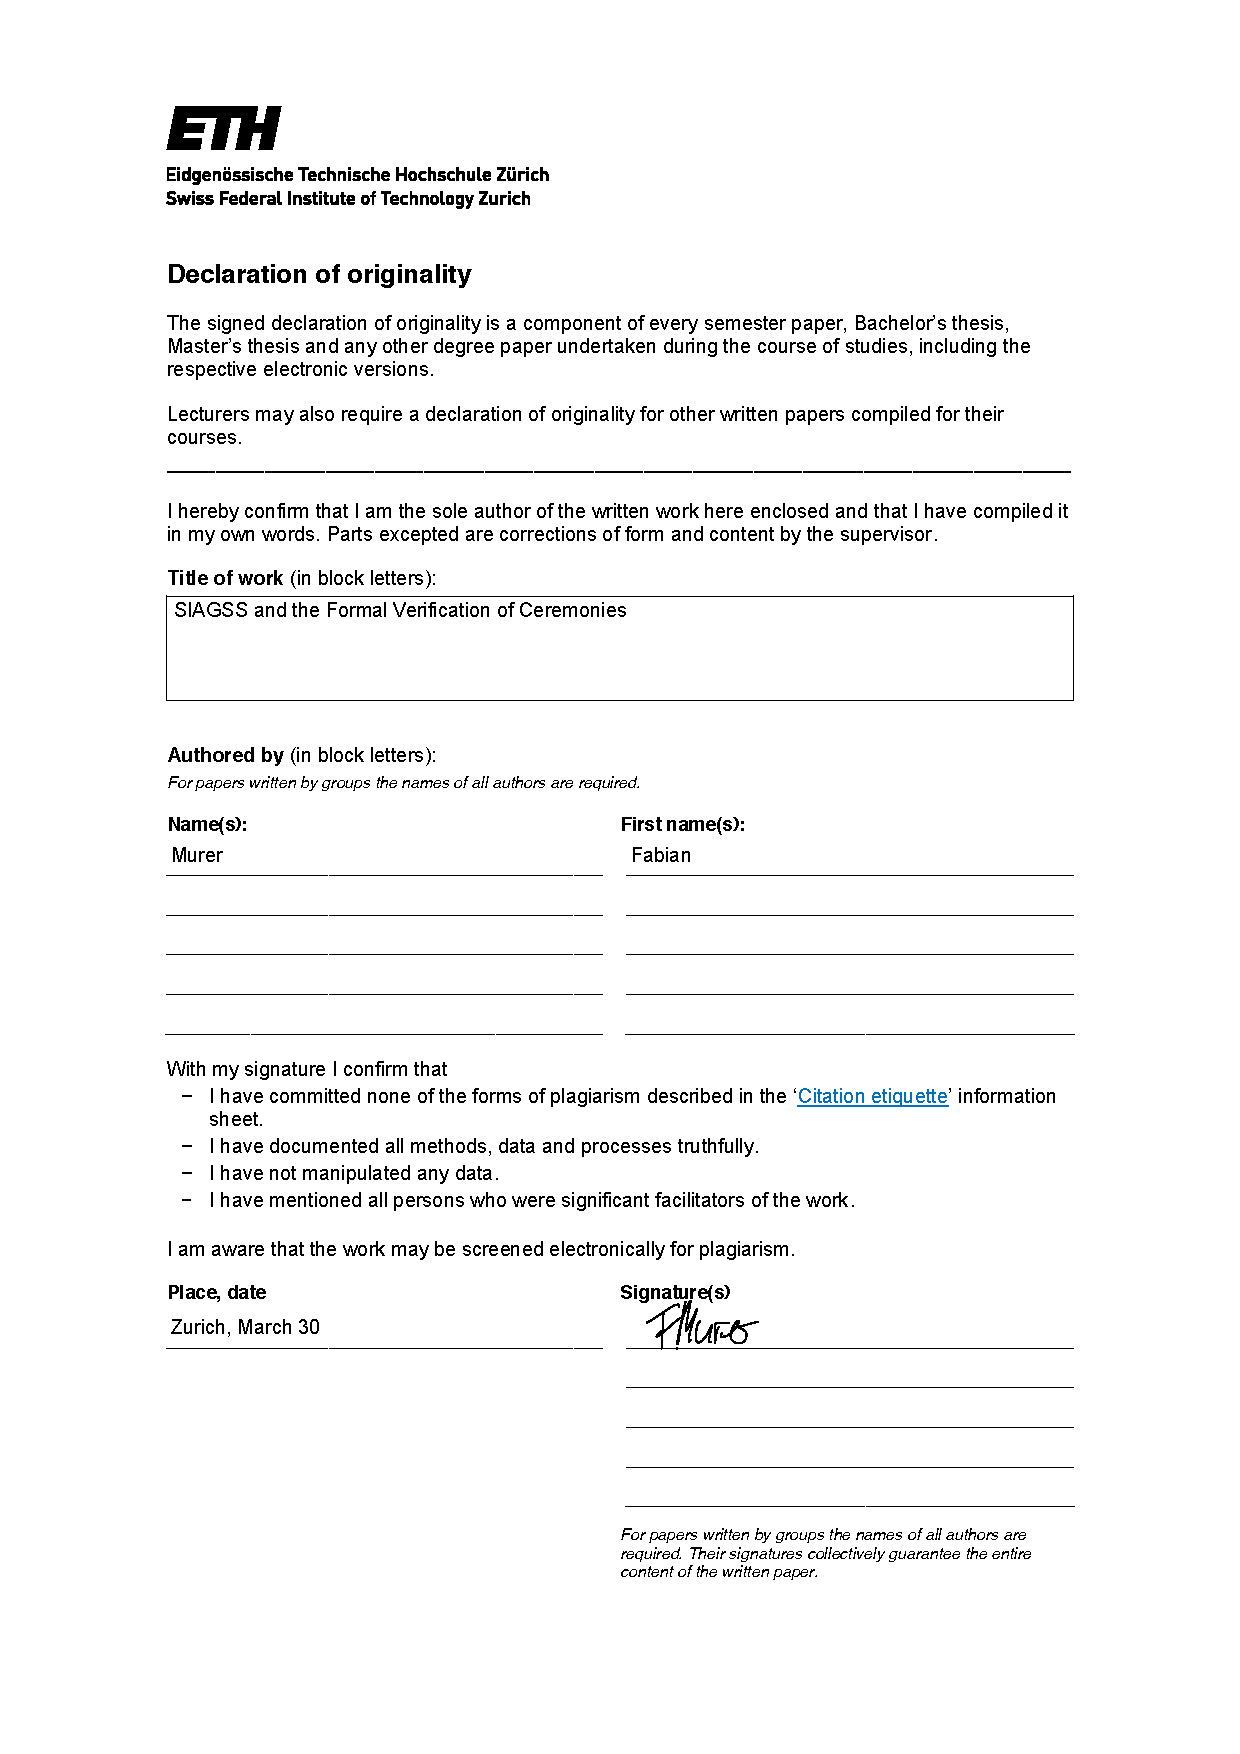
\includepdf[pages={-}]{declaration-originality.pdf}

\end{document}
